\section{Introduction}
\label{sec_intro}
\add{Monitoring the construction of buildings requires estimating the \textit{as-built} state and comparing it with} the \textit{as-planned} design, typically represented as a Building Information Model (BIM)~\cite{bim}, which encodes the structural layout, including walls, floors, and other architectural elements.
Enabling applications such as on-site progress tracking and Augmented Reality (AR) visualization on portable devices~\cite{yigitbas2023supportingAR} requires real-time estimation and continuous updating of the \textit{as-built} state.
\add{Visual Simultaneous Localization and Mapping (Visual SLAM) provides a framework for jointly reconstructing the environment and localizing the sensor~\cite{cadena2016past}.}


\change{However, visual SLAM remains vulnerable to the characteristics of construction environments. Repetitive layouts, large textureless surfaces, and occlusions introduce ambiguous observations that accumulate as trajectory drift, producing maps that are geometrically inaccurate with the actual environment and limit their reliability for monitoring~\cite{sun2025nothingHilti}.}
{However, visual SLAM remains prone to trajectory drift in construction environments, where ambiguous observations accumulate as localization error throughout the trajectory~\cite{sun2025nothingHilti}, producing maps that are geometrically inaccurate with the actual environment, directly compromising the reliability of \textit{as-built} vs.\ \textit{as-planned} comparisons essential for progress tracking.}
\add{Incorporating architectural priors from the BIM into the SLAM pipeline offers the possibility to enforce structural consistency and mitigate drift. Such integration has been investigated in LiDAR-based systems~\cite{isgraphs} that operate in indoor environments where structural elements are already in place and can be matched against the prior. However, to the best of our knowledge, architectural BIM priors have not yet been explicitly embedded within a visual SLAM framework. This integration is non-trivial in the visual domain. Sparser, range-limited depth and higher per-frame noise lead to greater drift accumulation, which in turn complicates the association between detected walls and their BIM counterparts.}


\begin{figure}[t]
    \centering
    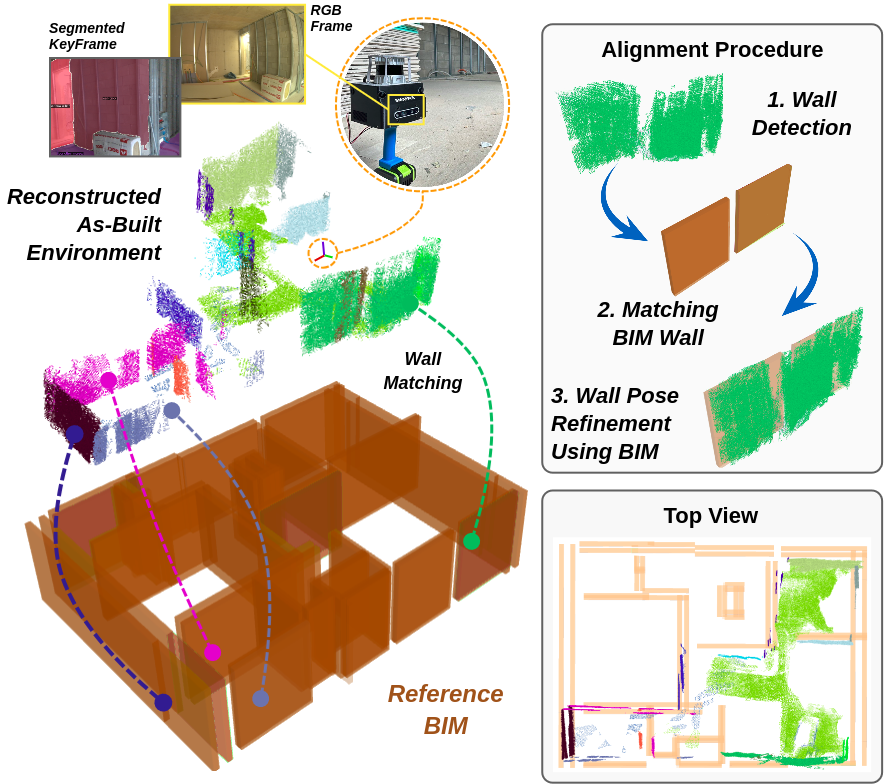
\includegraphics[width=0.9\columnwidth]{Figures/Overview_smapper_VS-Graphs.png}
    \caption{Proposed BIM-informed RGB-D SLAM system. Detected \textit{as-built} walls are matched to their \textit{as-planned} BIM counterparts, with a 2D projection of the alignment.}
    \label{fig:front_image}
\end{figure}



To fill this gap, this work proposes \textit{ivS-Graphs} (illustrated in Fig.~\ref{fig:front_image}), building upon an existing visual SLAM backbone~\cite{tourani2025vsgraphs} that jointly estimates structural planes with keyframe poses. 
\add{ivS-Graphs extends this backbone by introducing BIM walls as prior nodes and matching them against locally detected walls, aligning the evolving map with the \textit{as-planned} design and reducing drift throughout the trajectory.}
\change{Walls are chosen as the key structural element because they are among the earliest and most persistent features in construction environments, providing reliable geometric anchors even under partial observability.}
{\addtwo{The system targets indoor, wall-dominant, building construction environments, such as residential buildings, where walls are among the earliest and most persistent planar features, providing reliable geometric anchors even under partial observability. They are therefore chosen as the key structural element for correspondence with the BIM.}}
The main contributions of this work are:

\begin{itemize}
    \item A novel integration of architectural BIM priors into a visual SLAM framework, reducing trajectory drift by enforcing structural consistency between the \textit{as-built} map and the \textit{as-planned} BIM.
    \item A wall-based initialization and association strategy that establishes correspondences between \textit{as-planned} and \textit{as-built} walls using only two walls as prior information, enabling deployment from the earliest stages of operation.
    \item A system that maintains mapping accuracy under partially built conditions and geometric discrepancies between the \textit{as-planned} and \textit{as-built} models.
\end{itemize}


